\documentclass[1p]{elsarticle_modified}
%\bibliographystyle{elsarticle-num}

%\usepackage[colorlinks]{hyperref}
%\usepackage{abbrmath_seonhwa} %\Abb, \Ascr, \Acal ,\Abf, \Afrak
\usepackage{amsfonts}
\usepackage{amssymb}
\usepackage{amsmath}
\usepackage{amsthm}
\usepackage{scalefnt}
\usepackage{amsbsy}
\usepackage{kotex}
\usepackage{caption}
\usepackage{subfig}
\usepackage{color}
\usepackage{graphicx}
\usepackage{xcolor} %% white, black, red, green, blue, cyan, magenta, yellow
\usepackage{float}
\usepackage{setspace}
\usepackage{hyperref}

\usepackage{tikz}
\usetikzlibrary{arrows}

\usepackage{multirow}
\usepackage{array} % fixed length table
\usepackage{hhline}

%%%%%%%%%%%%%%%%%%%%%
\makeatletter
\renewcommand*\env@matrix[1][\arraystretch]{%
	\edef\arraystretch{#1}%
	\hskip -\arraycolsep
	\let\@ifnextchar\new@ifnextchar
	\array{*\c@MaxMatrixCols c}}
\makeatother %https://tex.stackexchange.com/questions/14071/how-can-i-increase-the-line-spacing-in-a-matrix
%%%%%%%%%%%%%%%

\usepackage[normalem]{ulem}

\newcommand{\msout}[1]{\ifmmode\text{\sout{\ensuremath{#1}}}\else\sout{#1}\fi}
%SOURCE: \msout is \stkout macro in https://tex.stackexchange.com/questions/20609/strikeout-in-math-mode

\newcommand{\cancel}[1]{
	\ifmmode
	{\color{red}\msout{#1}}
	\else
	{\color{red}\sout{#1}}
	\fi
}

\newcommand{\add}[1]{
	{\color{blue}\uwave{#1}}
}

\newcommand{\replace}[2]{
	\ifmmode
	{\color{red}\msout{#1}}{\color{blue}\uwave{#2}}
	\else
	{\color{red}\sout{#1}}{\color{blue}\uwave{#2}}
	\fi
}

\newcommand{\Sol}{\mathcal{S}} %segment
\newcommand{\D}{D} %diagram
\newcommand{\A}{\mathcal{A}} %arc


%%%%%%%%%%%%%%%%%%%%%%%%%%%%%5 test

\def\sl{\operatorname{\textup{SL}}(2,\Cbb)}
\def\psl{\operatorname{\textup{PSL}}(2,\Cbb)}
\def\quan{\mkern 1mu \triangleright \mkern 1mu}

\theoremstyle{definition}
\newtheorem{thm}{Theorem}[section]
\newtheorem{prop}[thm]{Proposition}
\newtheorem{lem}[thm]{Lemma}
\newtheorem{ques}[thm]{Question}
\newtheorem{cor}[thm]{Corollary}
\newtheorem{defn}[thm]{Definition}
\newtheorem{exam}[thm]{Example}
\newtheorem{rmk}[thm]{Remark}
\newtheorem{alg}[thm]{Algorithm}

\newcommand{\I}{\sqrt{-1}}
\begin{document}

%\begin{frontmatter}
%
%\title{Boundary parabolic representations of knots up to 8 crossings}
%
%%% Group authors per affiliation:
%\author{Yunhi Cho} 
%\address{Department of Mathematics, University of Seoul, Seoul, Korea}
%\ead{yhcho@uos.ac.kr}
%
%
%\author{Seonhwa Kim} %\fnref{s_kim}}
%\address{Center for Geometry and Physics, Institute for Basic Science, Pohang, 37673, Korea}
%\ead{ryeona17@ibs.re.kr}
%
%\author{Hyuk Kim}
%\address{Department of Mathematical Sciences, Seoul National University, Seoul 08826, Korea}
%\ead{hyukkim@snu.ac.kr}
%
%\author{Seokbeom Yoon}
%\address{Department of Mathematical Sciences, Seoul National University, Seoul, 08826,  Korea}
%\ead{sbyoon15@snu.ac.kr}
%
%\begin{abstract}
%We find all boundary parabolic representation of knots up to 8 crossings.
%
%\end{abstract}
%\begin{keyword}
%    \MSC[2010] 57M25 
%\end{keyword}
%
%\end{frontmatter}

%\linenumbers
%\tableofcontents
%
\newcommand\colored[1]{\textcolor{white}{\rule[-0.35ex]{0.8em}{1.4ex}}\kern-0.8em\color{red} #1}%
%\newcommand\colored[1]{\textcolor{white}{ #1}\kern-2.17ex	\textcolor{white}{ #1}\kern-1.81ex	\textcolor{white}{ #1}\kern-2.15ex\color{red}#1	}

{\Large $\underline{12n_{0747}~(K12n_{0747})}$}

\setlength{\tabcolsep}{10pt}
\renewcommand{\arraystretch}{1.6}
\vspace{1cm}\begin{tabular}{m{100pt}>{\centering\arraybackslash}m{274pt}}
\multirow{5}{120pt}{
	\centering
	\includegraphics[width=112pt]{../../../GIT/diagram.site/Diagrams/png/2836_12n_0747.png}\\
\ \ \ A knot diagram\footnotemark}&
\allowdisplaybreaks
\textbf{Linearized knot diagam} \\
\cline{2-2}
 &
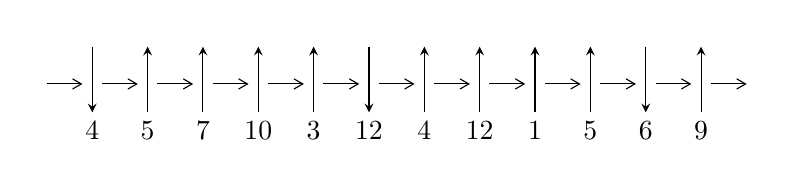
\begin{tikzpicture}[x=20pt, y=17pt]
	% nodes
	\node (C0) at (0, 0) {};
	\node (C1) at (1, 0) {};
	\node (C1U) at (1, +1) {};
	\node (C1D) at (1, -1) {4};

	\node (C2) at (2, 0) {};
	\node (C2U) at (2, +1) {};
	\node (C2D) at (2, -1) {5};

	\node (C3) at (3, 0) {};
	\node (C3U) at (3, +1) {};
	\node (C3D) at (3, -1) {7};

	\node (C4) at (4, 0) {};
	\node (C4U) at (4, +1) {};
	\node (C4D) at (4, -1) {10};

	\node (C5) at (5, 0) {};
	\node (C5U) at (5, +1) {};
	\node (C5D) at (5, -1) {3};

	\node (C6) at (6, 0) {};
	\node (C6U) at (6, +1) {};
	\node (C6D) at (6, -1) {12};

	\node (C7) at (7, 0) {};
	\node (C7U) at (7, +1) {};
	\node (C7D) at (7, -1) {4};

	\node (C8) at (8, 0) {};
	\node (C8U) at (8, +1) {};
	\node (C8D) at (8, -1) {12};

	\node (C9) at (9, 0) {};
	\node (C9U) at (9, +1) {};
	\node (C9D) at (9, -1) {1};

	\node (C10) at (10, 0) {};
	\node (C10U) at (10, +1) {};
	\node (C10D) at (10, -1) {5};

	\node (C11) at (11, 0) {};
	\node (C11U) at (11, +1) {};
	\node (C11D) at (11, -1) {6};

	\node (C12) at (12, 0) {};
	\node (C12U) at (12, +1) {};
	\node (C12D) at (12, -1) {9};
	\node (C13) at (13, 0) {};

	% arrows
	\draw[->,>={angle 60}]
	(C0) edge (C1) (C1) edge (C2) (C2) edge (C3) (C3) edge (C4) (C4) edge (C5) (C5) edge (C6) (C6) edge (C7) (C7) edge (C8) (C8) edge (C9) (C9) edge (C10) (C10) edge (C11) (C11) edge (C12) (C12) edge (C13) ;	\draw[->,>=stealth]
	(C1U) edge (C1D) (C2D) edge (C2U) (C3D) edge (C3U) (C4D) edge (C4U) (C5D) edge (C5U) (C6U) edge (C6D) (C7D) edge (C7U) (C8D) edge (C8U) (C9D) edge (C9U) (C10D) edge (C10U) (C11U) edge (C11D) (C12D) edge (C12U) ;
	\end{tikzpicture} \\
\hhline{~~} \\& 
\textbf{Solving Sequence} \\ \cline{2-2} 
 &
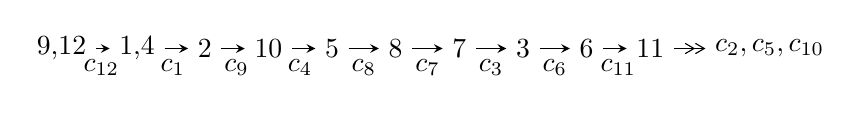
\begin{tikzpicture}[x=23pt, y=7pt]
	% node
	\node (A0) at (-1/8, 0) {9,12};
	\node (A1) at (17/16, 0) {1,4};
	\node (A2) at (17/8, 0) {2};
	\node (A3) at (25/8, 0) {10};
	\node (A4) at (33/8, 0) {5};
	\node (A5) at (41/8, 0) {8};
	\node (A6) at (49/8, 0) {7};
	\node (A7) at (57/8, 0) {3};
	\node (A8) at (65/8, 0) {6};
	\node (A9) at (73/8, 0) {11};
	\node (C1) at (1/2, -1) {$c_{12}$};
	\node (C2) at (13/8, -1) {$c_{1}$};
	\node (C3) at (21/8, -1) {$c_{9}$};
	\node (C4) at (29/8, -1) {$c_{4}$};
	\node (C5) at (37/8, -1) {$c_{8}$};
	\node (C6) at (45/8, -1) {$c_{7}$};
	\node (C7) at (53/8, -1) {$c_{3}$};
	\node (C8) at (61/8, -1) {$c_{6}$};
	\node (C9) at (69/8, -1) {$c_{11}$};
	\node (A10) at (11, 0) {$c_{2},c_{5},c_{10}$};

	% edge
	\draw[->,>=stealth]	
	(A0) edge (A1) (A1) edge (A2) (A2) edge (A3) (A3) edge (A4) (A4) edge (A5) (A5) edge (A6) (A6) edge (A7) (A7) edge (A8) (A8) edge (A9) ;
	\draw[->>,>={angle 60}]	
	(A9) edge (A10);
\end{tikzpicture} \\ 

\end{tabular} \\

\footnotetext{
The image of knot diagram is generated by the software ``\textbf{Draw programme}" developed by Andrew Bartholomew(\url{http://www.layer8.co.uk/maths/draw/index.htm\#Running-draw}), where we modified some parts for our purpose(\url{https://github.com/CATsTAILs/LinksPainter}).
}\phantom \\ \newline 
\centering \textbf{Ideals for irreducible components\footnotemark of $X_{\text{par}}$} 
 
\begin{align*}
I^u_{1}&=\langle 
-2.18510\times10^{87} u^{63}+3.43048\times10^{87} u^{62}+\cdots+1.06222\times10^{86} b+4.40024\times10^{87},\\
\phantom{I^u_{1}}&\phantom{= \langle  }1.30342\times10^{88} u^{63}-1.96828\times10^{88} u^{62}+\cdots+1.06222\times10^{86} a-2.56911\times10^{88},\;u^{64}-2 u^{63}+\cdots-23 u+1\rangle \\
I^u_{2}&=\langle 
u^5- u^4-3 u^3+u^2+b+2 u+1,\;2 u^9-2 u^8-12 u^7+9 u^6+24 u^5-11 u^4-17 u^3+a+2 u+6,\\
\phantom{I^u_{2}}&\phantom{= \langle  }u^{10}- u^9-6 u^8+4 u^7+13 u^6-4 u^5-11 u^4-2 u^3+2 u^2+4 u+1\rangle \\
I^u_{3}&=\langle 
b+a+u+1,\;a^2+a u+3 a+u+1,\;u^2+u-1\rangle \\
\\
\end{align*}
\raggedright * 3 irreducible components of $\dim_{\mathbb{C}}=0$, with total 78 representations.\\
\footnotetext{All coefficients of polynomials are rational numbers. But the coefficients are sometimes approximated in decimal forms when there is not enough margin.}
\newpage
\renewcommand{\arraystretch}{1}
\centering \section*{I. $I^u_{1}= \langle -2.19\times10^{87} u^{63}+3.43\times10^{87} u^{62}+\cdots+1.06\times10^{86} b+4.40\times10^{87},\;1.30\times10^{88} u^{63}-1.97\times10^{88} u^{62}+\cdots+1.06\times10^{86} a-2.57\times10^{88},\;u^{64}-2 u^{63}+\cdots-23 u+1 \rangle$}
\flushleft \textbf{(i) Arc colorings}\\
\begin{tabular}{m{7pt} m{180pt} m{7pt} m{180pt} }
\flushright $a_{9}=$&$\begin{pmatrix}0\\u\end{pmatrix}$ \\
\flushright $a_{12}=$&$\begin{pmatrix}1\\0\end{pmatrix}$ \\
\flushright $a_{1}=$&$\begin{pmatrix}1\\- u^2\end{pmatrix}$ \\
\flushright $a_{4}=$&$\begin{pmatrix}-122.708 u^{63}+185.299 u^{62}+\cdots-5249.53 u+241.862\\20.5711 u^{63}-32.2954 u^{62}+\cdots+884.457 u-41.4249\end{pmatrix}$ \\
\flushright $a_{2}=$&$\begin{pmatrix}80.9216 u^{63}-120.495 u^{62}+\cdots+3818.05 u-185.936\\-10.4054 u^{63}+15.9135 u^{62}+\cdots-498.812 u+22.3121\end{pmatrix}$ \\
\flushright $a_{10}=$&$\begin{pmatrix}u\\- u^3+u\end{pmatrix}$ \\
\flushright $a_{5}=$&$\begin{pmatrix}-97.7534 u^{63}+145.797 u^{62}+\cdots-4117.81 u+187.718\\42.6309 u^{63}-64.8314 u^{62}+\cdots+1801.77 u-85.1621\end{pmatrix}$ \\
\flushright $a_{8}=$&$\begin{pmatrix}- u\\u\end{pmatrix}$ \\
\flushright $a_{7}=$&$\begin{pmatrix}-44.4529 u^{63}+65.0075 u^{62}+\cdots-1944.92 u+88.7000\\-21.8652 u^{63}+33.1776 u^{62}+\cdots-951.044 u+46.6180\end{pmatrix}$ \\
\flushright $a_{3}=$&$\begin{pmatrix}148.216 u^{63}-219.442 u^{62}+\cdots+6319.96 u-310.655\\-26.4978 u^{63}+40.7839 u^{62}+\cdots-1214.82 u+58.2926\end{pmatrix}$ \\
\flushright $a_{6}=$&$\begin{pmatrix}-66.3181 u^{63}+98.1851 u^{62}+\cdots-2895.96 u+135.318\\-21.8652 u^{63}+33.1776 u^{62}+\cdots-951.044 u+46.6180\end{pmatrix}$ \\
\flushright $a_{11}=$&$\begin{pmatrix}-17.7302 u^{63}+25.0723 u^{62}+\cdots-616.299 u+35.7654\\51.1592 u^{63}-77.8247 u^{62}+\cdots+2236.56 u-107.971\end{pmatrix}$\\&\end{tabular}
\flushleft \textbf{(ii) Obstruction class $= -1$}\\~\\
\flushleft \textbf{(iii) Cusp Shapes $= 812.905 u^{63}-1227.04 u^{62}+\cdots+34392.6 u-1624.68$}\\~\\
\newpage\renewcommand{\arraystretch}{1}
\flushleft \textbf{(iv) u-Polynomials at the component}\newline \\
\begin{tabular}{m{50pt}|m{274pt}}
Crossings & \hspace{64pt}u-Polynomials at each crossing \\
\hline $$\begin{aligned}c_{1}\end{aligned}$$&$\begin{aligned}
&u^{64}-6 u^{63}+\cdots+392 u+49
\end{aligned}$\\
\hline $$\begin{aligned}c_{2},c_{5}\end{aligned}$$&$\begin{aligned}
&u^{64}-2 u^{63}+\cdots+14 u+1
\end{aligned}$\\
\hline $$\begin{aligned}c_{3},c_{7}\end{aligned}$$&$\begin{aligned}
&u^{64}- u^{63}+\cdots-30 u+7
\end{aligned}$\\
\hline $$\begin{aligned}c_{4},c_{10}\end{aligned}$$&$\begin{aligned}
&u^{64}-2 u^{63}+\cdots-649 u-23
\end{aligned}$\\
\hline $$\begin{aligned}c_{6},c_{11}\end{aligned}$$&$\begin{aligned}
&u^{64}- u^{63}+\cdots+16 u+1
\end{aligned}$\\
\hline $$\begin{aligned}c_{8},c_{9},c_{12}\end{aligned}$$&$\begin{aligned}
&u^{64}-2 u^{63}+\cdots-23 u+1
\end{aligned}$\\
\hline
\end{tabular}\\~\\
\newpage\renewcommand{\arraystretch}{1}
\flushleft \textbf{(v) Riley Polynomials at the component}\newline \\
\begin{tabular}{m{50pt}|m{274pt}}
Crossings & \hspace{64pt}Riley Polynomials at each crossing \\
\hline $$\begin{aligned}c_{1}\end{aligned}$$&$\begin{aligned}
&y^{64}-10 y^{63}+\cdots-254506 y+2401
\end{aligned}$\\
\hline $$\begin{aligned}c_{2},c_{5}\end{aligned}$$&$\begin{aligned}
&y^{64}-18 y^{63}+\cdots-60 y+1
\end{aligned}$\\
\hline $$\begin{aligned}c_{3},c_{7}\end{aligned}$$&$\begin{aligned}
&y^{64}-21 y^{63}+\cdots-3056 y+49
\end{aligned}$\\
\hline $$\begin{aligned}c_{4},c_{10}\end{aligned}$$&$\begin{aligned}
&y^{64}-28 y^{63}+\cdots-464395 y+529
\end{aligned}$\\
\hline $$\begin{aligned}c_{6},c_{11}\end{aligned}$$&$\begin{aligned}
&y^{64}-51 y^{63}+\cdots-312 y+1
\end{aligned}$\\
\hline $$\begin{aligned}c_{8},c_{9},c_{12}\end{aligned}$$&$\begin{aligned}
&y^{64}-58 y^{63}+\cdots+39 y+1
\end{aligned}$\\
\hline
\end{tabular}\\~\\
\newpage\flushleft \textbf{(vi) Complex Volumes and Cusp Shapes}
$$\begin{array}{c|c|c}  
\text{Solutions to }I^u_{1}& \I (\text{vol} + \sqrt{-1}CS) & \text{Cusp shape}\\
 \hline 
\begin{aligned}
u &= \phantom{-}0.145672 + 0.968068 I \\
a &= \phantom{-}0.158850 - 0.010710 I \\
b &= -0.509053 + 0.675145 I\end{aligned}
 & \phantom{-}1.07637 + 4.19054 I & \phantom{-0.000000 } 0 \\ \hline\begin{aligned}
u &= \phantom{-}0.145672 - 0.968068 I \\
a &= \phantom{-}0.158850 + 0.010710 I \\
b &= -0.509053 - 0.675145 I\end{aligned}
 & \phantom{-}1.07637 - 4.19054 I & \phantom{-0.000000 } 0 \\ \hline\begin{aligned}
u &= -0.317235 + 1.010710 I \\
a &= -0.0311390 + 0.0511144 I \\
b &= -1.146370 - 0.672425 I\end{aligned}
 & -4.56279 - 10.69090 I & \phantom{-0.000000 } 0 \\ \hline\begin{aligned}
u &= -0.317235 - 1.010710 I \\
a &= -0.0311390 - 0.0511144 I \\
b &= -1.146370 + 0.672425 I\end{aligned}
 & -4.56279 + 10.69090 I & \phantom{-0.000000 } 0 \\ \hline\begin{aligned}
u &= -0.317994 + 0.869749 I \\
a &= \phantom{-}0.0728894 + 0.0793513 I \\
b &= \phantom{-}1.254910 + 0.487312 I\end{aligned}
 & -6.15152 - 3.00155 I & \phantom{-0.000000 } 0 \\ \hline\begin{aligned}
u &= -0.317994 - 0.869749 I \\
a &= \phantom{-}0.0728894 - 0.0793513 I \\
b &= \phantom{-}1.254910 - 0.487312 I\end{aligned}
 & -6.15152 + 3.00155 I & \phantom{-0.000000 } 0 \\ \hline\begin{aligned}
u &= -0.950390 + 0.519722 I \\
a &= \phantom{-}0.594935 + 1.039960 I \\
b &= -0.623717 + 0.052076 I\end{aligned}
 & -4.21641 - 1.93351 I & \phantom{-0.000000 } 0 \\ \hline\begin{aligned}
u &= -0.950390 - 0.519722 I \\
a &= \phantom{-}0.594935 - 1.039960 I \\
b &= -0.623717 - 0.052076 I\end{aligned}
 & -4.21641 + 1.93351 I & \phantom{-0.000000 } 0 \\ \hline\begin{aligned}
u &= -0.017192 + 0.901588 I \\
a &= \phantom{-}0.068027 + 0.657514 I \\
b &= -1.070960 + 0.469701 I\end{aligned}
 & -5.87061 + 3.95242 I & \phantom{-0.000000 } 0 \\ \hline\begin{aligned}
u &= -0.017192 - 0.901588 I \\
a &= \phantom{-}0.068027 - 0.657514 I \\
b &= -1.070960 - 0.469701 I\end{aligned}
 & -5.87061 - 3.95242 I & \phantom{-0.000000 } 0\\
 \hline 
 \end{array}$$\newpage$$\begin{array}{c|c|c}  
\text{Solutions to }I^u_{1}& \I (\text{vol} + \sqrt{-1}CS) & \text{Cusp shape}\\
 \hline 
\begin{aligned}
u &= \phantom{-}1.076120 + 0.259760 I \\
a &= \phantom{-}0.82530 + 1.41539 I \\
b &= -0.22338 - 1.44415 I\end{aligned}
 & \phantom{-}2.60826 + 0.73468 I & \phantom{-0.000000 } 0 \\ \hline\begin{aligned}
u &= \phantom{-}1.076120 - 0.259760 I \\
a &= \phantom{-}0.82530 - 1.41539 I \\
b &= -0.22338 + 1.44415 I\end{aligned}
 & \phantom{-}2.60826 - 0.73468 I & \phantom{-0.000000 } 0 \\ \hline\begin{aligned}
u &= \phantom{-}0.045996 + 0.875054 I \\
a &= \phantom{-}0.201918 - 0.847332 I \\
b &= \phantom{-}1.087860 - 0.197488 I\end{aligned}
 & -4.71214 - 3.22971 I & \phantom{-0.000000 } 0 \\ \hline\begin{aligned}
u &= \phantom{-}0.045996 - 0.875054 I \\
a &= \phantom{-}0.201918 + 0.847332 I \\
b &= \phantom{-}1.087860 + 0.197488 I\end{aligned}
 & -4.71214 + 3.22971 I & \phantom{-0.000000 } 0 \\ \hline\begin{aligned}
u &= \phantom{-}1.149260 + 0.077977 I \\
a &= -0.74710 + 1.82542 I \\
b &= \phantom{-}1.69518 - 1.61779 I\end{aligned}
 & \phantom{-}3.76038 + 0.86686 I & \phantom{-0.000000 } 0 \\ \hline\begin{aligned}
u &= \phantom{-}1.149260 - 0.077977 I \\
a &= -0.74710 - 1.82542 I \\
b &= \phantom{-}1.69518 + 1.61779 I\end{aligned}
 & \phantom{-}3.76038 - 0.86686 I & \phantom{-0.000000 } 0 \\ \hline\begin{aligned}
u &= \phantom{-}1.16929\phantom{ +0.000000I} \\
a &= -0.910966\phantom{ +0.000000I} \\
b &= -0.966261\phantom{ +0.000000I}\end{aligned}
 & \phantom{-}8.52254\phantom{ +0.000000I} & \phantom{-0.000000 } 0 \\ \hline\begin{aligned}
u &= -0.936704 + 0.797768 I \\
a &= -0.469421 - 0.560340 I \\
b &= \phantom{-}0.560431 - 0.288250 I\end{aligned}
 & -2.68573 + 4.64400 I & \phantom{-0.000000 } 0 \\ \hline\begin{aligned}
u &= -0.936704 - 0.797768 I \\
a &= -0.469421 + 0.560340 I \\
b &= \phantom{-}0.560431 + 0.288250 I\end{aligned}
 & -2.68573 - 4.64400 I & \phantom{-0.000000 } 0 \\ \hline\begin{aligned}
u &= \phantom{-}1.222740 + 0.203951 I \\
a &= \phantom{-}0.695120 - 0.912173 I \\
b &= -1.110160 + 0.648732 I\end{aligned}
 & \phantom{-}1.76600 + 0.88415 I & \phantom{-0.000000 } 0\\
 \hline 
 \end{array}$$\newpage$$\begin{array}{c|c|c}  
\text{Solutions to }I^u_{1}& \I (\text{vol} + \sqrt{-1}CS) & \text{Cusp shape}\\
 \hline 
\begin{aligned}
u &= \phantom{-}1.222740 - 0.203951 I \\
a &= \phantom{-}0.695120 + 0.912173 I \\
b &= -1.110160 - 0.648732 I\end{aligned}
 & \phantom{-}1.76600 - 0.88415 I & \phantom{-0.000000 } 0 \\ \hline\begin{aligned}
u &= -1.246660 + 0.059464 I \\
a &= -0.55090 - 1.49771 I \\
b &= -0.171764 + 0.903029 I\end{aligned}
 & \phantom{-}5.22128 + 0.20023 I & \phantom{-0.000000 } 0 \\ \hline\begin{aligned}
u &= -1.246660 - 0.059464 I \\
a &= -0.55090 + 1.49771 I \\
b &= -0.171764 - 0.903029 I\end{aligned}
 & \phantom{-}5.22128 - 0.20023 I & \phantom{-0.000000 } 0 \\ \hline\begin{aligned}
u &= \phantom{-}1.272690 + 0.032209 I \\
a &= \phantom{-}0.15479 - 2.26835 I \\
b &= -0.88983 + 1.50685 I\end{aligned}
 & \phantom{-}3.53094 + 4.77456 I & \phantom{-0.000000 } 0 \\ \hline\begin{aligned}
u &= \phantom{-}1.272690 - 0.032209 I \\
a &= \phantom{-}0.15479 + 2.26835 I \\
b &= -0.88983 - 1.50685 I\end{aligned}
 & \phantom{-}3.53094 - 4.77456 I & \phantom{-0.000000 } 0 \\ \hline\begin{aligned}
u &= \phantom{-}0.088214 + 0.702646 I \\
a &= \phantom{-}0.445527 + 0.157220 I \\
b &= \phantom{-}0.698844 - 0.817971 I\end{aligned}
 & -0.19370 + 2.61233 I & \phantom{-}7.84382 - 3.48904 I \\ \hline\begin{aligned}
u &= \phantom{-}0.088214 - 0.702646 I \\
a &= \phantom{-}0.445527 - 0.157220 I \\
b &= \phantom{-}0.698844 + 0.817971 I\end{aligned}
 & -0.19370 - 2.61233 I & \phantom{-}7.84382 + 3.48904 I \\ \hline\begin{aligned}
u &= \phantom{-}1.240250 + 0.395827 I \\
a &= \phantom{-}0.50755 - 1.33041 I \\
b &= -0.398132 + 0.148486 I\end{aligned}
 & -1.02699 + 7.77383 I & \phantom{-0.000000 } 0 \\ \hline\begin{aligned}
u &= \phantom{-}1.240250 - 0.395827 I \\
a &= \phantom{-}0.50755 + 1.33041 I \\
b &= -0.398132 - 0.148486 I\end{aligned}
 & -1.02699 - 7.77383 I & \phantom{-0.000000 } 0 \\ \hline\begin{aligned}
u &= -1.300310 + 0.106200 I \\
a &= \phantom{-}0.10878 + 2.07536 I \\
b &= \phantom{-}0.21246 - 1.86082 I\end{aligned}
 & \phantom{-}4.03767 - 5.60876 I & \phantom{-0.000000 } 0\\
 \hline 
 \end{array}$$\newpage$$\begin{array}{c|c|c}  
\text{Solutions to }I^u_{1}& \I (\text{vol} + \sqrt{-1}CS) & \text{Cusp shape}\\
 \hline 
\begin{aligned}
u &= -1.300310 - 0.106200 I \\
a &= \phantom{-}0.10878 - 2.07536 I \\
b &= \phantom{-}0.21246 + 1.86082 I\end{aligned}
 & \phantom{-}4.03767 + 5.60876 I & \phantom{-0.000000 } 0 \\ \hline\begin{aligned}
u &= \phantom{-}0.127283 + 0.672520 I \\
a &= -0.046765 + 0.488251 I \\
b &= \phantom{-}1.054710 - 0.369106 I\end{aligned}
 & -1.43385 + 2.27144 I & \phantom{-}1.22544 - 3.26874 I \\ \hline\begin{aligned}
u &= \phantom{-}0.127283 - 0.672520 I \\
a &= -0.046765 - 0.488251 I \\
b &= \phantom{-}1.054710 + 0.369106 I\end{aligned}
 & -1.43385 - 2.27144 I & \phantom{-}1.22544 + 3.26874 I \\ \hline\begin{aligned}
u &= -1.266290 + 0.418664 I \\
a &= -0.46184 - 1.34292 I \\
b &= \phantom{-}1.53300 + 1.08160 I\end{aligned}
 & -1.99825 - 8.66191 I & \phantom{-0.000000 } 0 \\ \hline\begin{aligned}
u &= -1.266290 - 0.418664 I \\
a &= -0.46184 + 1.34292 I \\
b &= \phantom{-}1.53300 - 1.08160 I\end{aligned}
 & -1.99825 + 8.66191 I & \phantom{-0.000000 } 0 \\ \hline\begin{aligned}
u &= \phantom{-}1.261270 + 0.461738 I \\
a &= -0.471642 - 0.784639 I \\
b &= -0.246549 + 0.646298 I\end{aligned}
 & \phantom{-}4.61034 + 1.14842 I & \phantom{-0.000000 } 0 \\ \hline\begin{aligned}
u &= \phantom{-}1.261270 - 0.461738 I \\
a &= -0.471642 + 0.784639 I \\
b &= -0.246549 - 0.646298 I\end{aligned}
 & \phantom{-}4.61034 - 1.14842 I & \phantom{-0.000000 } 0 \\ \hline\begin{aligned}
u &= -1.323370 + 0.315223 I \\
a &= -0.00992 + 1.87693 I \\
b &= -0.84124 - 1.24795 I\end{aligned}
 & \phantom{-}4.22712 - 6.35841 I & \phantom{-0.000000 } 0 \\ \hline\begin{aligned}
u &= -1.323370 - 0.315223 I \\
a &= -0.00992 - 1.87693 I \\
b &= -0.84124 + 1.24795 I\end{aligned}
 & \phantom{-}4.22712 + 6.35841 I & \phantom{-0.000000 } 0 \\ \hline\begin{aligned}
u &= \phantom{-}1.290860 + 0.454754 I \\
a &= -0.544269 + 0.810497 I \\
b &= \phantom{-}0.318363 + 0.015687 I\end{aligned}
 & -1.80259 + 0.89192 I & \phantom{-0.000000 } 0\\
 \hline 
 \end{array}$$\newpage$$\begin{array}{c|c|c}  
\text{Solutions to }I^u_{1}& \I (\text{vol} + \sqrt{-1}CS) & \text{Cusp shape}\\
 \hline 
\begin{aligned}
u &= \phantom{-}1.290860 - 0.454754 I \\
a &= -0.544269 - 0.810497 I \\
b &= \phantom{-}0.318363 - 0.015687 I\end{aligned}
 & -1.80259 - 0.89192 I & \phantom{-0.000000 } 0 \\ \hline\begin{aligned}
u &= -1.37057\phantom{ +0.000000I} \\
a &= -0.961744\phantom{ +0.000000I} \\
b &= -0.218443\phantom{ +0.000000I}\end{aligned}
 & \phantom{-}8.24072\phantom{ +0.000000I} & \phantom{-0.000000 } 0 \\ \hline\begin{aligned}
u &= -1.306900 + 0.427782 I \\
a &= \phantom{-}0.534404 + 0.813965 I \\
b &= -1.58618 - 0.60287 I\end{aligned}
 & -0.48910 - 1.44438 I & \phantom{-0.000000 } 0 \\ \hline\begin{aligned}
u &= -1.306900 - 0.427782 I \\
a &= \phantom{-}0.534404 - 0.813965 I \\
b &= -1.58618 + 0.60287 I\end{aligned}
 & -0.48910 + 1.44438 I & \phantom{-0.000000 } 0 \\ \hline\begin{aligned}
u &= -1.366280 + 0.266791 I \\
a &= \phantom{-}0.53978 + 1.75105 I \\
b &= -0.88158 - 1.25458 I\end{aligned}
 & \phantom{-}3.30380 - 5.68458 I & \phantom{-0.000000 } 0 \\ \hline\begin{aligned}
u &= -1.366280 - 0.266791 I \\
a &= \phantom{-}0.53978 - 1.75105 I \\
b &= -0.88158 + 1.25458 I\end{aligned}
 & \phantom{-}3.30380 + 5.68458 I & \phantom{-0.000000 } 0 \\ \hline\begin{aligned}
u &= -1.38190 + 0.42110 I \\
a &= -0.02647 - 1.49795 I \\
b &= \phantom{-}0.78691 + 1.35385 I\end{aligned}
 & \phantom{-}5.89179 - 9.11420 I & \phantom{-0.000000 } 0 \\ \hline\begin{aligned}
u &= -1.38190 - 0.42110 I \\
a &= -0.02647 + 1.49795 I \\
b &= \phantom{-}0.78691 - 1.35385 I\end{aligned}
 & \phantom{-}5.89179 + 9.11420 I & \phantom{-0.000000 } 0 \\ \hline\begin{aligned}
u &= \phantom{-}0.553755\phantom{ +0.000000I} \\
a &= \phantom{-}1.04389\phantom{ +0.000000I} \\
b &= -0.735717\phantom{ +0.000000I}\end{aligned}
 & \phantom{-}1.07870\phantom{ +0.000000I} & \phantom{-}9.45760\phantom{ +0.000000I} \\ \hline\begin{aligned}
u &= -0.517206\phantom{ +0.000000I} \\
a &= -1.23311\phantom{ +0.000000I} \\
b &= -0.969631\phantom{ +0.000000I}\end{aligned}
 & \phantom{-}2.29968\phantom{ +0.000000I} & -3.88090\phantom{ +0.000000I}\\
 \hline 
 \end{array}$$\newpage$$\begin{array}{c|c|c}  
\text{Solutions to }I^u_{1}& \I (\text{vol} + \sqrt{-1}CS) & \text{Cusp shape}\\
 \hline 
\begin{aligned}
u &= \phantom{-}0.493387\phantom{ +0.000000I} \\
a &= -3.44102\phantom{ +0.000000I} \\
b &= \phantom{-}0.0313711\phantom{ +0.000000I}\end{aligned}
 & \phantom{-}6.36082\phantom{ +0.000000I} & \phantom{-}23.1340\phantom{ +0.000000I} \\ \hline\begin{aligned}
u &= \phantom{-}0.490027\phantom{ +0.000000I} \\
a &= \phantom{-}3.42978\phantom{ +0.000000I} \\
b &= -1.25784\phantom{ +0.000000I}\end{aligned}
 & \phantom{-}2.53719\phantom{ +0.000000I} & -23.9910\phantom{ +0.000000I} \\ \hline\begin{aligned}
u &= \phantom{-}1.49141 + 0.35489 I \\
a &= \phantom{-}0.78851 - 1.38211 I \\
b &= -1.63953 + 1.04123 I\end{aligned}
 & -0.31770 + 7.46862 I & \phantom{-0.000000 } 0 \\ \hline\begin{aligned}
u &= \phantom{-}1.49141 - 0.35489 I \\
a &= \phantom{-}0.78851 + 1.38211 I \\
b &= -1.63953 - 1.04123 I\end{aligned}
 & -0.31770 - 7.46862 I & \phantom{-0.000000 } 0 \\ \hline\begin{aligned}
u &= \phantom{-}1.47502 + 0.42826 I \\
a &= -0.46070 + 1.53329 I \\
b &= \phantom{-}1.42814 - 1.18260 I\end{aligned}
 & \phantom{-}1.1028 + 15.8670 I & \phantom{-0.000000 } 0 \\ \hline\begin{aligned}
u &= \phantom{-}1.47502 - 0.42826 I \\
a &= -0.46070 - 1.53329 I \\
b &= \phantom{-}1.42814 + 1.18260 I\end{aligned}
 & \phantom{-}1.1028 - 15.8670 I & \phantom{-0.000000 } 0 \\ \hline\begin{aligned}
u &= -1.54760\phantom{ +0.000000I} \\
a &= -0.228222\phantom{ +0.000000I} \\
b &= \phantom{-}1.16480\phantom{ +0.000000I}\end{aligned}
 & \phantom{-}13.5060\phantom{ +0.000000I} & \phantom{-0.000000 } 0 \\ \hline\begin{aligned}
u &= \phantom{-}1.62930\phantom{ +0.000000I} \\
a &= -1.54611\phantom{ +0.000000I} \\
b &= \phantom{-}2.23107\phantom{ +0.000000I}\end{aligned}
 & \phantom{-}10.1076\phantom{ +0.000000I} & \phantom{-0.000000 } 0 \\ \hline\begin{aligned}
u &= -1.64577\phantom{ +0.000000I} \\
a &= -1.16219\phantom{ +0.000000I} \\
b &= \phantom{-}1.38735\phantom{ +0.000000I}\end{aligned}
 & \phantom{-}9.05367\phantom{ +0.000000I} & \phantom{-0.000000 } 0 \\ \hline\begin{aligned}
u &= \phantom{-}0.175687 + 0.165118 I \\
a &= \phantom{-}2.69632 - 1.12663 I \\
b &= -0.541818 - 0.646762 I\end{aligned}
 & \phantom{-}1.211640 + 0.322145 I & \phantom{-}9.95422 - 2.34487 I\\
 \hline 
 \end{array}$$\newpage$$\begin{array}{c|c|c}  
\text{Solutions to }I^u_{1}& \I (\text{vol} + \sqrt{-1}CS) & \text{Cusp shape}\\
 \hline 
\begin{aligned}
u &= \phantom{-}0.175687 - 0.165118 I \\
a &= \phantom{-}2.69632 + 1.12663 I \\
b &= -0.541818 + 0.646762 I\end{aligned}
 & \phantom{-}1.211640 - 0.322145 I & \phantom{-}9.95422 + 2.34487 I \\ \hline\begin{aligned}
u &= \phantom{-}0.0579910 + 0.0764411 I \\
a &= -8.09290 + 2.32584 I \\
b &= \phantom{-}0.33102 - 1.44442 I\end{aligned}
 & -0.33025 + 4.70984 I & \phantom{-}11.3417 - 11.5444 I \\ \hline\begin{aligned}
u &= \phantom{-}0.0579910 - 0.0764411 I \\
a &= -8.09290 - 2.32584 I \\
b &= \phantom{-}0.33102 + 1.44442 I\end{aligned}
 & -0.33025 - 4.70984 I & \phantom{-}11.3417 + 11.5444 I \\ \hline\begin{aligned}
u &= \phantom{-}1.96691\phantom{ +0.000000I} \\
a &= \phantom{-}0.0504349\phantom{ +0.000000I} \\
b &= \phantom{-}0.170188\phantom{ +0.000000I}\end{aligned}
 & \phantom{-}7.42639\phantom{ +0.000000I} & \phantom{-0.000000 } 0\\
 \hline 
 \end{array}$$\newpage\newpage\renewcommand{\arraystretch}{1}
\centering \section*{II. $I^u_{2}= \langle u^5- u^4-3 u^3+u^2+b+2 u+1,\;2 u^9-2 u^8+\cdots+a+6,\;u^{10}- u^9+\cdots+4 u+1 \rangle$}
\flushleft \textbf{(i) Arc colorings}\\
\begin{tabular}{m{7pt} m{180pt} m{7pt} m{180pt} }
\flushright $a_{9}=$&$\begin{pmatrix}0\\u\end{pmatrix}$ \\
\flushright $a_{12}=$&$\begin{pmatrix}1\\0\end{pmatrix}$ \\
\flushright $a_{1}=$&$\begin{pmatrix}1\\- u^2\end{pmatrix}$ \\
\flushright $a_{4}=$&$\begin{pmatrix}-2 u^9+2 u^8+12 u^7-9 u^6-24 u^5+11 u^4+17 u^3-2 u-6\\- u^5+u^4+3 u^3- u^2-2 u-1\end{pmatrix}$ \\
\flushright $a_{2}=$&$\begin{pmatrix}2 u^8-5 u^7-5 u^6+17 u^5+u^4-14 u^3+u^2-2 u+6\\u^9-2 u^8-4 u^7+8 u^6+5 u^5-9 u^4-3 u^3+u^2+2 u+1\end{pmatrix}$ \\
\flushright $a_{10}=$&$\begin{pmatrix}u\\- u^3+u\end{pmatrix}$ \\
\flushright $a_{5}=$&$\begin{pmatrix}- u^9+8 u^7-2 u^6-18 u^5+5 u^4+13 u^3- u^2-5\\u^8- u^7-4 u^6+2 u^5+5 u^4+u^3- u^2-3 u-1\end{pmatrix}$ \\
\flushright $a_{8}=$&$\begin{pmatrix}- u\\u\end{pmatrix}$ \\
\flushright $a_{7}=$&$\begin{pmatrix}2 u^9-2 u^8-14 u^7+12 u^6+32 u^5-20 u^4-27 u^3+4 u^2+4 u+11\\u^9- u^8-5 u^7+3 u^6+9 u^5-2 u^4-6 u^3- u^2+u+1\end{pmatrix}$ \\
\flushright $a_{3}=$&$\begin{pmatrix}2 u^9-17 u^7+4 u^6+42 u^5-11 u^4-34 u^3+2 u^2+u+13\\u^9-2 u^8-4 u^7+8 u^6+5 u^5-9 u^4-2 u^3+u^2+u+1\end{pmatrix}$ \\
\flushright $a_{6}=$&$\begin{pmatrix}3 u^9-3 u^8-19 u^7+15 u^6+41 u^5-22 u^4-33 u^3+3 u^2+5 u+12\\u^9- u^8-5 u^7+3 u^6+9 u^5-2 u^4-6 u^3- u^2+u+1\end{pmatrix}$ \\
\flushright $a_{11}=$&$\begin{pmatrix}-3 u^9+5 u^8+15 u^7-21 u^6-28 u^5+26 u^4+22 u^3-2 u^2-7 u-9\\- u^3+2 u\end{pmatrix}$\\&\end{tabular}
\flushleft \textbf{(ii) Obstruction class $= 1$}\\~\\
\flushleft \textbf{(iii) Cusp Shapes $= -7 u^9+12 u^8+30 u^7-45 u^6-46 u^5+43 u^4+32 u^3+10 u^2-15 u-6$}\\~\\
\newpage\renewcommand{\arraystretch}{1}
\flushleft \textbf{(iv) u-Polynomials at the component}\newline \\
\begin{tabular}{m{50pt}|m{274pt}}
Crossings & \hspace{64pt}u-Polynomials at each crossing \\
\hline $$\begin{aligned}c_{1}\end{aligned}$$&$\begin{aligned}
&u^{10}+u^9+u^8+16 u^7+11 u^6+11 u^5+27 u^4+13 u^3+3 u^2-1
\end{aligned}$\\
\hline $$\begin{aligned}c_{2}\end{aligned}$$&$\begin{aligned}
&u^{10}+u^9-3 u^8-6 u^7-2 u^6+7 u^5+9 u^4+3 u^3-4 u^2-4 u-1
\end{aligned}$\\
\hline $$\begin{aligned}c_{3}\end{aligned}$$&$\begin{aligned}
&u^{10}-6 u^9+13 u^8-11 u^7-2 u^6+12 u^5-7 u^4-5 u^3+8 u^2-5 u+1
\end{aligned}$\\
\hline $$\begin{aligned}c_{4}\end{aligned}$$&$\begin{aligned}
&u^{10}-3 u^8+u^7+2 u^6-2 u^5+u^4+u^3-2 u^2- u+1
\end{aligned}$\\
\hline $$\begin{aligned}c_{5}\end{aligned}$$&$\begin{aligned}
&u^{10}- u^9-3 u^8+6 u^7-2 u^6-7 u^5+9 u^4-3 u^3-4 u^2+4 u-1
\end{aligned}$\\
\hline $$\begin{aligned}c_{6}\end{aligned}$$&$\begin{aligned}
&u^{10}+u^9-2 u^8- u^7+u^6+2 u^5+2 u^4- u^3-3 u^2+1
\end{aligned}$\\
\hline $$\begin{aligned}c_{7}\end{aligned}$$&$\begin{aligned}
&u^{10}+6 u^9+13 u^8+11 u^7-2 u^6-12 u^5-7 u^4+5 u^3+8 u^2+5 u+1
\end{aligned}$\\
\hline $$\begin{aligned}c_{8},c_{9}\end{aligned}$$&$\begin{aligned}
&u^{10}+u^9-6 u^8-4 u^7+13 u^6+4 u^5-11 u^4+2 u^3+2 u^2-4 u+1
\end{aligned}$\\
\hline $$\begin{aligned}c_{10}\end{aligned}$$&$\begin{aligned}
&u^{10}-3 u^8- u^7+2 u^6+2 u^5+u^4- u^3-2 u^2+u+1
\end{aligned}$\\
\hline $$\begin{aligned}c_{11}\end{aligned}$$&$\begin{aligned}
&u^{10}- u^9-2 u^8+u^7+u^6-2 u^5+2 u^4+u^3-3 u^2+1
\end{aligned}$\\
\hline $$\begin{aligned}c_{12}\end{aligned}$$&$\begin{aligned}
&u^{10}- u^9-6 u^8+4 u^7+13 u^6-4 u^5-11 u^4-2 u^3+2 u^2+4 u+1
\end{aligned}$\\
\hline
\end{tabular}\\~\\
\newpage\renewcommand{\arraystretch}{1}
\flushleft \textbf{(v) Riley Polynomials at the component}\newline \\
\begin{tabular}{m{50pt}|m{274pt}}
Crossings & \hspace{64pt}Riley Polynomials at each crossing \\
\hline $$\begin{aligned}c_{1}\end{aligned}$$&$\begin{aligned}
&y^{10}+y^9+\cdots-6 y+1
\end{aligned}$\\
\hline $$\begin{aligned}c_{2},c_{5}\end{aligned}$$&$\begin{aligned}
&y^{10}-7 y^9+\cdots-8 y+1
\end{aligned}$\\
\hline $$\begin{aligned}c_{3},c_{7}\end{aligned}$$&$\begin{aligned}
&y^{10}-10 y^9+33 y^8-43 y^7+42 y^6-76 y^5+53 y^4-21 y^3-9 y+1
\end{aligned}$\\
\hline $$\begin{aligned}c_{4},c_{10}\end{aligned}$$&$\begin{aligned}
&y^{10}-6 y^9+13 y^8-11 y^7-2 y^6+12 y^5-7 y^4-5 y^3+8 y^2-5 y+1
\end{aligned}$\\
\hline $$\begin{aligned}c_{6},c_{11}\end{aligned}$$&$\begin{aligned}
&y^{10}-5 y^9+8 y^8-5 y^7-7 y^6+12 y^5-2 y^4-11 y^3+13 y^2-6 y+1
\end{aligned}$\\
\hline $$\begin{aligned}c_{8},c_{9},c_{12}\end{aligned}$$&$\begin{aligned}
&y^{10}-13 y^9+\cdots-12 y+1
\end{aligned}$\\
\hline
\end{tabular}\\~\\
\newpage\flushleft \textbf{(vi) Complex Volumes and Cusp Shapes}
$$\begin{array}{c|c|c}  
\text{Solutions to }I^u_{2}& \I (\text{vol} + \sqrt{-1}CS) & \text{Cusp shape}\\
 \hline 
\begin{aligned}
u &= \phantom{-}1.118050 + 0.232448 I \\
a &= -0.159280 - 1.307010 I \\
b &= -0.630949 + 1.176290 I\end{aligned}
 & \phantom{-}3.06671 + 1.14968 I & \phantom{-}12.41669 - 0.09656 I \\ \hline\begin{aligned}
u &= \phantom{-}1.118050 - 0.232448 I \\
a &= -0.159280 + 1.307010 I \\
b &= -0.630949 - 1.176290 I\end{aligned}
 & \phantom{-}3.06671 - 1.14968 I & \phantom{-}12.41669 + 0.09656 I \\ \hline\begin{aligned}
u &= -1.27546\phantom{ +0.000000I} \\
a &= -1.36835\phantom{ +0.000000I} \\
b &= -0.278715\phantom{ +0.000000I}\end{aligned}
 & \phantom{-}9.38465\phantom{ +0.000000I} & \phantom{-}20.1760\phantom{ +0.000000I} \\ \hline\begin{aligned}
u &= -1.333980 + 0.226517 I \\
a &= \phantom{-}0.35319 + 2.32281 I \\
b &= -0.92049 - 1.72482 I\end{aligned}
 & \phantom{-}3.07640 - 6.89606 I & \phantom{-}7.33660 + 9.72380 I \\ \hline\begin{aligned}
u &= -1.333980 - 0.226517 I \\
a &= \phantom{-}0.35319 - 2.32281 I \\
b &= -0.92049 + 1.72482 I\end{aligned}
 & \phantom{-}3.07640 + 6.89606 I & \phantom{-}7.33660 - 9.72380 I \\ \hline\begin{aligned}
u &= -0.227124 + 0.579101 I \\
a &= \phantom{-}0.242833 + 0.178690 I \\
b &= \phantom{-}0.488743 - 1.032260 I\end{aligned}
 & -0.76904 + 4.14977 I & \phantom{-}4.72090 - 3.87430 I \\ \hline\begin{aligned}
u &= -0.227124 - 0.579101 I \\
a &= \phantom{-}0.242833 - 0.178690 I \\
b &= \phantom{-}0.488743 + 1.032260 I\end{aligned}
 & -0.76904 - 4.14977 I & \phantom{-}4.72090 + 3.87430 I \\ \hline\begin{aligned}
u &= \phantom{-}1.55280\phantom{ +0.000000I} \\
a &= -0.492950\phantom{ +0.000000I} \\
b &= \phantom{-}1.50160\phantom{ +0.000000I}\end{aligned}
 & \phantom{-}12.6171\phantom{ +0.000000I} & \phantom{-}9.76370\phantom{ +0.000000I} \\ \hline\begin{aligned}
u &= -0.288130\phantom{ +0.000000I} \\
a &= -5.71392\phantom{ +0.000000I} \\
b &= -0.569642\phantom{ +0.000000I}\end{aligned}
 & \phantom{-}6.02399\phantom{ +0.000000I} & -1.25560\phantom{ +0.000000I} \\ \hline\begin{aligned}
u &= \phantom{-}1.89689\phantom{ +0.000000I} \\
a &= -0.298260\phantom{ +0.000000I} \\
b &= \phantom{-}0.472157\phantom{ +0.000000I}\end{aligned}
 & \phantom{-}7.28432\phantom{ +0.000000I} & -12.6330\phantom{ +0.000000I}\\
 \hline 
 \end{array}$$\newpage\newpage\renewcommand{\arraystretch}{1}
\centering \section*{III. $I^u_{3}= \langle b+a+u+1,\;a^2+a u+3 a+u+1,\;u^2+u-1 \rangle$}
\flushleft \textbf{(i) Arc colorings}\\
\begin{tabular}{m{7pt} m{180pt} m{7pt} m{180pt} }
\flushright $a_{9}=$&$\begin{pmatrix}0\\u\end{pmatrix}$ \\
\flushright $a_{12}=$&$\begin{pmatrix}1\\0\end{pmatrix}$ \\
\flushright $a_{1}=$&$\begin{pmatrix}1\\u-1\end{pmatrix}$ \\
\flushright $a_{4}=$&$\begin{pmatrix}a\\- a- u-1\end{pmatrix}$ \\
\flushright $a_{2}=$&$\begin{pmatrix}a u+2\\- a u+a+2 u\end{pmatrix}$ \\
\flushright $a_{10}=$&$\begin{pmatrix}u\\- u+1\end{pmatrix}$ \\
\flushright $a_{5}=$&$\begin{pmatrix}- a u+a- u\\a u-2 a-2\end{pmatrix}$ \\
\flushright $a_{8}=$&$\begin{pmatrix}- u\\u\end{pmatrix}$ \\
\flushright $a_{7}=$&$\begin{pmatrix}a- u\\- a-1\end{pmatrix}$ \\
\flushright $a_{3}=$&$\begin{pmatrix}u\\- u\end{pmatrix}$ \\
\flushright $a_{6}=$&$\begin{pmatrix}- u-1\\- a-1\end{pmatrix}$ \\
\flushright $a_{11}=$&$\begin{pmatrix}- a u- a- u\\a u+a+u\end{pmatrix}$\\&\end{tabular}
\flushleft \textbf{(ii) Obstruction class $= 1$}\\~\\
\flushleft \textbf{(iii) Cusp Shapes $= -6 a u-13 a-2 u+14$}\\~\\
\newpage\renewcommand{\arraystretch}{1}
\flushleft \textbf{(iv) u-Polynomials at the component}\newline \\
\begin{tabular}{m{50pt}|m{274pt}}
Crossings & \hspace{64pt}u-Polynomials at each crossing \\
\hline $$\begin{aligned}c_{1},c_{2}\end{aligned}$$&$\begin{aligned}
&u^4+2 u^3-2 u^2-3 u+1
\end{aligned}$\\
\hline $$\begin{aligned}c_{3}\end{aligned}$$&$\begin{aligned}
&(u+1)^4
\end{aligned}$\\
\hline $$\begin{aligned}c_{4},c_{6}\end{aligned}$$&$\begin{aligned}
&u^4+u^3-3 u^2- u+1
\end{aligned}$\\
\hline $$\begin{aligned}c_{5}\end{aligned}$$&$\begin{aligned}
&u^4-2 u^3-2 u^2+3 u+1
\end{aligned}$\\
\hline $$\begin{aligned}c_{7}\end{aligned}$$&$\begin{aligned}
&(u-1)^4
\end{aligned}$\\
\hline $$\begin{aligned}c_{8},c_{9}\end{aligned}$$&$\begin{aligned}
&(u^2- u-1)^2
\end{aligned}$\\
\hline $$\begin{aligned}c_{10},c_{11}\end{aligned}$$&$\begin{aligned}
&u^4- u^3-3 u^2+u+1
\end{aligned}$\\
\hline $$\begin{aligned}c_{12}\end{aligned}$$&$\begin{aligned}
&(u^2+u-1)^2
\end{aligned}$\\
\hline
\end{tabular}\\~\\
\newpage\renewcommand{\arraystretch}{1}
\flushleft \textbf{(v) Riley Polynomials at the component}\newline \\
\begin{tabular}{m{50pt}|m{274pt}}
Crossings & \hspace{64pt}Riley Polynomials at each crossing \\
\hline $$\begin{aligned}c_{1},c_{2},c_{5}\end{aligned}$$&$\begin{aligned}
&y^4-8 y^3+18 y^2-13 y+1
\end{aligned}$\\
\hline $$\begin{aligned}c_{3},c_{7}\end{aligned}$$&$\begin{aligned}
&(y-1)^4
\end{aligned}$\\
\hline $$\begin{aligned}c_{4},c_{6},c_{10}\\c_{11}\end{aligned}$$&$\begin{aligned}
&y^4-7 y^3+13 y^2-7 y+1
\end{aligned}$\\
\hline $$\begin{aligned}c_{8},c_{9},c_{12}\end{aligned}$$&$\begin{aligned}
&(y^2-3 y+1)^2
\end{aligned}$\\
\hline
\end{tabular}\\~\\
\newpage\flushleft \textbf{(vi) Complex Volumes and Cusp Shapes}
$$\begin{array}{c|c|c}  
\text{Solutions to }I^u_{3}& \I (\text{vol} + \sqrt{-1}CS) & \text{Cusp shape}\\
 \hline 
\begin{aligned}
u &= \phantom{-}0.618034\phantom{ +0.000000I} \\
a &= -0.522740\phantom{ +0.000000I} \\
b &= -1.09529\phantom{ +0.000000I}\end{aligned}
 & \phantom{-}2.63189\phantom{ +0.000000I} & \phantom{-}21.4980\phantom{ +0.000000I} \\ \hline\begin{aligned}
u &= \phantom{-}0.618034\phantom{ +0.000000I} \\
a &= -3.09529\phantom{ +0.000000I} \\
b &= \phantom{-}1.47726\phantom{ +0.000000I}\end{aligned}
 & \phantom{-}2.63189\phantom{ +0.000000I} & \phantom{-}64.4810\phantom{ +0.000000I} \\ \hline\begin{aligned}
u &= -1.61803\phantom{ +0.000000I} \\
a &= \phantom{-}0.355674\phantom{ +0.000000I} \\
b &= \phantom{-}0.262360\phantom{ +0.000000I}\end{aligned}
 & \phantom{-}10.5276\phantom{ +0.000000I} & \phantom{-}16.0650\phantom{ +0.000000I} \\ \hline\begin{aligned}
u &= -1.61803\phantom{ +0.000000I} \\
a &= -1.73764\phantom{ +0.000000I} \\
b &= \phantom{-}2.35567\phantom{ +0.000000I}\end{aligned}
 & \phantom{-}10.5276\phantom{ +0.000000I} & \phantom{-}22.9560\phantom{ +0.000000I}\\
 \hline 
 \end{array}$$\newpage
\newpage\renewcommand{\arraystretch}{1}
\centering \section*{ IV. u-Polynomials}
\begin{tabular}{m{50pt}|m{274pt}}
Crossings & \hspace{64pt}u-Polynomials at each crossing \\
\hline $$\begin{aligned}c_{1}\end{aligned}$$&$\begin{aligned}
&(u^4+2 u^3-2 u^2-3 u+1)\\
&\cdot(u^{10}+u^9+u^8+16 u^7+11 u^6+11 u^5+27 u^4+13 u^3+3 u^2-1)\\
&\cdot(u^{64}-6 u^{63}+\cdots+392 u+49)
\end{aligned}$\\
\hline $$\begin{aligned}c_{2}\end{aligned}$$&$\begin{aligned}
&(u^4+2 u^3-2 u^2-3 u+1)\\
&\cdot(u^{10}+u^9-3 u^8-6 u^7-2 u^6+7 u^5+9 u^4+3 u^3-4 u^2-4 u-1)\\
&\cdot(u^{64}-2 u^{63}+\cdots+14 u+1)
\end{aligned}$\\
\hline $$\begin{aligned}c_{3}\end{aligned}$$&$\begin{aligned}
&(u+1)^4\\
&\cdot(u^{10}-6 u^9+13 u^8-11 u^7-2 u^6+12 u^5-7 u^4-5 u^3+8 u^2-5 u+1)\\
&\cdot(u^{64}- u^{63}+\cdots-30 u+7)
\end{aligned}$\\
\hline $$\begin{aligned}c_{4}\end{aligned}$$&$\begin{aligned}
&(u^4+u^3-3 u^2- u+1)(u^{10}-3 u^8+\cdots- u+1)\\
&\cdot(u^{64}-2 u^{63}+\cdots-649 u-23)
\end{aligned}$\\
\hline $$\begin{aligned}c_{5}\end{aligned}$$&$\begin{aligned}
&(u^4-2 u^3-2 u^2+3 u+1)\\
&\cdot(u^{10}- u^9-3 u^8+6 u^7-2 u^6-7 u^5+9 u^4-3 u^3-4 u^2+4 u-1)\\
&\cdot(u^{64}-2 u^{63}+\cdots+14 u+1)
\end{aligned}$\\
\hline $$\begin{aligned}c_{6}\end{aligned}$$&$\begin{aligned}
&(u^4+u^3-3 u^2- u+1)\\
&\cdot(u^{10}+u^9-2 u^8- u^7+u^6+2 u^5+2 u^4- u^3-3 u^2+1)\\
&\cdot(u^{64}- u^{63}+\cdots+16 u+1)
\end{aligned}$\\
\hline $$\begin{aligned}c_{7}\end{aligned}$$&$\begin{aligned}
&(u-1)^4\\
&\cdot(u^{10}+6 u^9+13 u^8+11 u^7-2 u^6-12 u^5-7 u^4+5 u^3+8 u^2+5 u+1)\\
&\cdot(u^{64}- u^{63}+\cdots-30 u+7)
\end{aligned}$\\
\hline $$\begin{aligned}c_{8},c_{9}\end{aligned}$$&$\begin{aligned}
&(u^2- u-1)^2\\
&\cdot(u^{10}+u^9-6 u^8-4 u^7+13 u^6+4 u^5-11 u^4+2 u^3+2 u^2-4 u+1)\\
&\cdot(u^{64}-2 u^{63}+\cdots-23 u+1)
\end{aligned}$\\
\hline $$\begin{aligned}c_{10}\end{aligned}$$&$\begin{aligned}
&(u^4- u^3-3 u^2+u+1)(u^{10}-3 u^8+\cdots+u+1)\\
&\cdot(u^{64}-2 u^{63}+\cdots-649 u-23)
\end{aligned}$\\
\hline $$\begin{aligned}c_{11}\end{aligned}$$&$\begin{aligned}
&(u^4- u^3-3 u^2+u+1)\\
&\cdot(u^{10}- u^9-2 u^8+u^7+u^6-2 u^5+2 u^4+u^3-3 u^2+1)\\
&\cdot(u^{64}- u^{63}+\cdots+16 u+1)
\end{aligned}$\\
\hline $$\begin{aligned}c_{12}\end{aligned}$$&$\begin{aligned}
&(u^2+u-1)^2\\
&\cdot(u^{10}- u^9-6 u^8+4 u^7+13 u^6-4 u^5-11 u^4-2 u^3+2 u^2+4 u+1)\\
&\cdot(u^{64}-2 u^{63}+\cdots-23 u+1)
\end{aligned}$\\
\hline
\end{tabular}\newpage\renewcommand{\arraystretch}{1}
\centering \section*{ V. Riley Polynomials}
\begin{tabular}{m{50pt}|m{274pt}}
Crossings & \hspace{64pt}Riley Polynomials at each crossing \\
\hline $$\begin{aligned}c_{1}\end{aligned}$$&$\begin{aligned}
&(y^4-8 y^3+18 y^2-13 y+1)(y^{10}+y^9+\cdots-6 y+1)\\
&\cdot(y^{64}-10 y^{63}+\cdots-254506 y+2401)
\end{aligned}$\\
\hline $$\begin{aligned}c_{2},c_{5}\end{aligned}$$&$\begin{aligned}
&(y^4-8 y^3+18 y^2-13 y+1)(y^{10}-7 y^9+\cdots-8 y+1)\\
&\cdot(y^{64}-18 y^{63}+\cdots-60 y+1)
\end{aligned}$\\
\hline $$\begin{aligned}c_{3},c_{7}\end{aligned}$$&$\begin{aligned}
&(y-1)^4\\
&\cdot(y^{10}-10 y^9+33 y^8-43 y^7+42 y^6-76 y^5+53 y^4-21 y^3-9 y+1)\\
&\cdot(y^{64}-21 y^{63}+\cdots-3056 y+49)
\end{aligned}$\\
\hline $$\begin{aligned}c_{4},c_{10}\end{aligned}$$&$\begin{aligned}
&(y^4-7 y^3+13 y^2-7 y+1)\\
&\cdot(y^{10}-6 y^9+13 y^8-11 y^7-2 y^6+12 y^5-7 y^4-5 y^3+8 y^2-5 y+1)\\
&\cdot(y^{64}-28 y^{63}+\cdots-464395 y+529)
\end{aligned}$\\
\hline $$\begin{aligned}c_{6},c_{11}\end{aligned}$$&$\begin{aligned}
&(y^4-7 y^3+13 y^2-7 y+1)\\
&\cdot(y^{10}-5 y^9+8 y^8-5 y^7-7 y^6+12 y^5-2 y^4-11 y^3+13 y^2-6 y+1)\\
&\cdot(y^{64}-51 y^{63}+\cdots-312 y+1)
\end{aligned}$\\
\hline $$\begin{aligned}c_{8},c_{9},c_{12}\end{aligned}$$&$\begin{aligned}
&((y^2-3 y+1)^2)(y^{10}-13 y^9+\cdots-12 y+1)\\
&\cdot(y^{64}-58 y^{63}+\cdots+39 y+1)
\end{aligned}$\\
\hline
\end{tabular}
\vskip 2pc
\end{document}